% 图 4.3 超交换的自旋组态 (a)-(f) 与 M-O-M 轨道杂化示意
\documentclass[tikz,border=5pt]{standalone}
\usetikzlibrary{arrows.meta}
\usepackage{amsmath}
\usepackage{bm}
\usepackage{fontspec}
\setmainfont{Times New Roman}
\begin{document}
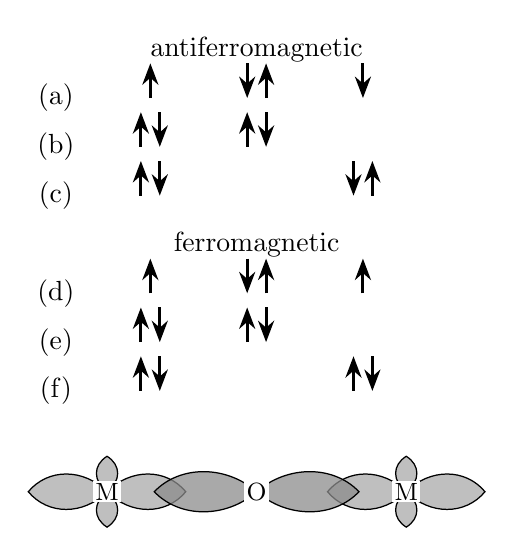
\begin{tikzpicture}[line width=0.8pt,>=Stealth]
\tikzset{
  up/.style={line width=1.05pt,->},
  dn/.style={line width=1.05pt,->},
  lobe/.style={line width=0.45pt}}
% single arrow at x, baseline y, direction #3 (1=up, -1=down)
\newcommand{\one}[3]{%
  \ifnum#3>0 \draw[up] (#1,#2) -- (#1,#2+0.44);
  \else      \draw[dn] (#1,#2+0.44) -- (#1,#2);\fi}
% pair at x, baseline y, order #3 (1 = up-down, -1 = down-up)
\newcommand{\pair}[3]{%
  \ifnum#3>0 \draw[up] (#1-0.12,#2) -- (#1-0.12,#2+0.44);
             \draw[dn] (#1+0.12,#2+0.44) -- (#1+0.12,#2);
  \else      \draw[dn] (#1-0.12,#2+0.44) -- (#1-0.12,#2);
             \draw[up] (#1+0.12,#2) -- (#1+0.12,#2+0.44);\fi}
% ---------- antiferromagnetic ----------
\node at (0,0.62) {antiferromagnetic};
\node at (-2.55,0) {(a)};  \one{-1.35}{0}{1}   \pair{0}{0}{-1}   \one{1.35}{0}{-1}
\node at (-2.55,-0.62) {(b)}; \pair{-1.35}{-0.62}{1} \pair{0}{-0.62}{1}
\node at (-2.55,-1.24) {(c)}; \pair{-1.35}{-1.24}{1} \pair{1.35}{-1.24}{-1}
% ---------- ferromagnetic ----------
\node at (0,-1.86) {ferromagnetic};
\node at (-2.55,-2.48) {(d)}; \one{-1.35}{-2.48}{1} \pair{0}{-2.48}{-1} \one{1.35}{-2.48}{1}
\node at (-2.55,-3.10) {(e)}; \pair{-1.35}{-3.10}{1} \pair{0}{-3.10}{1}
\node at (-2.55,-3.72) {(f)}; \pair{-1.35}{-3.72}{1} \pair{1.35}{-3.72}{1}
% ---------- M-O-M orbital overlap ----------
\newcommand{\lobe}[6]{% x, y, angle, length, half-width, style
  \begin{scope}[shift={(#1,#2)},rotate={#3}]
    \filldraw[#6,lobe] (0,0) .. controls (0.30*#4,#5) and (0.75*#4,#5)
      .. (#4,0) .. controls (0.75*#4,-#5) and (0.30*#4,-#5) .. (0,0) -- cycle;
  \end{scope}}
% left M d orbitals
\lobe{-1.9}{-5.0}{0}{1.0}{0.30}{fill=gray!50}
\lobe{-1.9}{-5.0}{180}{1.0}{0.30}{fill=gray!50}
\lobe{-1.9}{-5.0}{90}{0.45}{0.18}{fill=gray!50}
\lobe{-1.9}{-5.0}{270}{0.45}{0.18}{fill=gray!50}
% right M d orbitals
\lobe{1.9}{-5.0}{0}{1.0}{0.30}{fill=gray!50}
\lobe{1.9}{-5.0}{180}{1.0}{0.30}{fill=gray!50}
\lobe{1.9}{-5.0}{90}{0.45}{0.18}{fill=gray!50}
\lobe{1.9}{-5.0}{270}{0.45}{0.18}{fill=gray!50}
% central O p orbitals (lens-shaped overlap with the d lobes)
\lobe{0}{-5.0}{0}{1.3}{0.34}{fill=black!45,fill opacity=0.75}
\lobe{0}{-5.0}{180}{1.3}{0.34}{fill=black!45,fill opacity=0.75}
% atom labels
\node[fill=white,inner sep=0.8pt] at (-1.9,-5.0) {\small M};
\node[fill=white,inner sep=0.8pt] at (0,-5.0) {\small O};
\node[fill=white,inner sep=0.8pt] at (1.9,-5.0) {\small M};
\end{tikzpicture}
\end{document}
